% 刚体的静力平衡
% 静力平衡|合外力|刚体|合力矩

\pentry{动量定理\upref{PLaw}, 角动量定理\upref{AMLaw}}
\subsection{结论}
在任意参考系中,若刚体所受的合外力,合外力矩都为零,则刚体质心不动或匀速运动, 且刚体没有转动或绕质心做匀速转动.

\subsection{推导}
把刚体看做由许多质点组成,合外力为零时刚体动量守恒%未完成
,而动量等于质心的动量\upref{SysP}
$\bvec p_c = M_c \bvec v_c$,所以质心做匀速运动或不动.

刚体合外力矩为零时,质点系角动量守恒\upref{AMLaw},而角动量等于质心的角动量 $\bvec L_c =\bvec r_c\cross \bvec p_c$ 加质心系中的角动量(\autoref{AngMom_eq5}\upref{AngMom}). 当质心匀速运动或不动时质心的角动量不变,所以质心系中刚体的角动量也不变,所以刚体绕质心做匀速转动或不转动.

\begin{example}{}\label{RBSt_ex1}
如\autoref{RBSt_fig1}, 一个质量为 $m$ 的线轴被斜挂在墙上, 线轴与墙面的摩擦系数为 $\mu$,线轴的大圆半径为 $R$, 小圆半径为 $r$, 求当 $\alpha$ 满足什么条件时, 线轴才能不滑落.
\begin{figure}[ht]
\centering
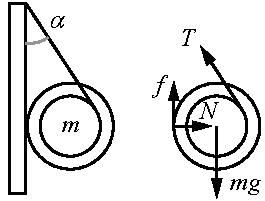
\includegraphics[width=4.3cm]{./figures/RBSt1.pdf}
\caption{线轴的平衡} \label{RBSt_fig1}
\end{figure}

我们先来看线轴受哪几个力:重力 $mg$, 绳的拉力 $T$, 墙的支持力 $N$ 和摩擦力 $f$. 由摩擦系数的定义和刚体平衡条件可得
\begin{equation}
\leftgroup{
&f \leqslant \mu N \quad \text{(摩擦系数)}\\
&N - T\sin\alpha = 0 \quad \text{(水平方向受力平衡)}\\
&T\cos\alpha + f - mg = 0 \quad \text{(竖直方向受力平衡)}\\
&Tr - fR = 0 \quad \text{(力矩平衡)}
}\end{equation}
其中最后一条力矩平衡是以圆心为原点计算力矩, 虽然原则上我们可以取任意点计算力矩, 但取在圆心计算最为简单. 除了 $\alpha$ 我们有三个未知数 $T, f, N$, 用以上三条等式恰好可以把这三个未知数消去, 可得关于 $\alpha$ 的不等式
\begin{equation}
\sin\alpha \ges \frac{r}{\mu R}
\end{equation}

一个有趣的地方在于, 不等式中没有出现质量 $m$. 事实上, 我们不使用那条含有 $mg$ 的等式也可以顺利得到答案.
\end{example}
